% ------------------------------------------------------------------
% Emi Compiler Documentation
% Generated from the project README plus a feature-by-feature walk
% of the compiler.
%
% This file holds the actual document; it is never compiled directly.
% main.tex (light) and dark.tex (dark) are thin wrappers that each
% \newif\ifemidark, set it, and \input this file - so the two PDFs
% share every word and only differ in the palette section below.
%
% Build with `make docs-pdf` from the repository root (builds both
% main.pdf and dark.pdf), or `make docs-pdf-light` / `make docs-pdf-dark`
% for just one. Directly: tectonic main.tex / tectonic dark.tex
% ------------------------------------------------------------------
\documentclass[10pt,a4paper]{extarticle}

\usepackage[margin=1.4cm,top=2.2cm,bottom=2cm]{geometry}
\usepackage{multicol}
\usepackage[T1]{fontenc}
\usepackage[utf8]{inputenc}
% ---------- O'Reilly-ish type: warm serif body, sans headings, ----------
% ---------- humanist monospace for code -------------------------------
\usepackage{mathpazo}                    % Palatino-based serif body text
\usepackage[scaled=0.92]{helvet}         % sans-serif for headings/rubrics
\usepackage[scaled=0.88]{inconsolata}    % humanist monospace for code
\usepackage{graphicx}
\usepackage{titlesec}
\usepackage{fancyhdr}
\usepackage{xcolor}
\usepackage{tcolorbox}
\usepackage{enumitem}
\usepackage{hyperref}
\usepackage{listings}
\usepackage{booktabs}
\usepackage{array}
\usepackage{ragged2e}
\usepackage{tikz}
\usetikzlibrary{arrows.meta,fit,backgrounds}

\tcbuselibrary{skins,breakable}

% ---------- palette (warm, book-ink tones) ----------
% \ifemidark is set by the wrapper file (main.tex / dark.tex) that
% \input this file - see the header comment above. Every other section
% in this document only ever refers to the named colors below (never a
% raw RGB triple), so the two builds differ only here.
\ifemidark
  \definecolor{paperbg}{RGB}{22,20,18}
  \definecolor{inkblack}{RGB}{230,224,216}
  \definecolor{rulegray}{RGB}{178,160,138}
  \definecolor{boxgray}{RGB}{42,38,33}
  \colorlet{panelbg}{paperbg}
  % ---------- per-section brand colours, brightened for a dark page ----------
  \definecolor{rustaccent}{RGB}{227,124,79}
  \definecolor{emipurple}{RGB}{191,142,224}
  \definecolor{goblue}{RGB}{104,181,227}
  \definecolor{jsyellow}{RGB}{216,178,66}
\else
  \definecolor{paperbg}{RGB}{255,255,255}
  \definecolor{inkblack}{RGB}{35,28,22}
  \definecolor{rulegray}{RGB}{150,132,110}
  \definecolor{boxgray}{RGB}{247,241,230}
  \colorlet{panelbg}{white}
  % ---------- per-section brand colours ----------
  \definecolor{rustaccent}{RGB}{176,68,24}
  \definecolor{emipurple}{RGB}{119,45,166}
  \definecolor{goblue}{RGB}{0,99,165}
  \definecolor{jsyellow}{RGB}{150,112,0}
\fi
\colorlet{accentcolor}{rustaccent}

\pagecolor{paperbg}
\color{inkblack}

% ---------- per-section colour themes ----------
% The book stays on this warm rust/ink palette by default, but three
% families of sections switch the accent colour and code-block tint to
% match what the section is actually about:
%   - rustaccent  : default / narrative sections (unchanged rust tone)
%   - emipurple   : the emi YAML/JSON definition itself (the "source of
%                   truth" you author, before any code generation happens)
%   - goblue      : sections about the generated Go server/client (Go's
%                   own brand blue, darkened for print contrast)
%   - jsyellow    : sections about the generated JS/TS client (JS's
%                   trademark yellow, darkened to stay legible as text)
% The tint/rule blend targets flip with the theme: light mode tints
% toward white and rules toward black; dark mode tints toward paperbg
% and rules toward white, so both stay legible on their own background.
\newcommand{\sectiontheme}[1]{%
  \colorlet{accentcolor}{#1}%
  \ifemidark
    \colorlet{boxgray}{#1!14!paperbg}%
    \colorlet{rulegray}{#1!55!white}%
  \else
    \colorlet{boxgray}{#1!6!white}%
    \colorlet{rulegray}{#1!45!black}%
  \fi
  \lstset{rulecolor=\color{rulegray}, backgroundcolor=\color{boxgray}}%
}

% ---------- heading fonts ----------
\newcommand{\headlinefont}{\normalfont\sffamily\bfseries\selectfont}
\titleformat{\section}{\headlinefont\Large\color{accentcolor}}{\thesection.}{0.4em}{}
\titlespacing*{\section}{0pt}{1.2ex plus .2ex minus .2ex}{0.6ex plus .1ex}
\titleformat{\subsection}{\headlinefont\normalsize\bfseries}{}{0em}{}
\titlespacing*{\subsection}{0pt}{1.4ex plus .4ex minus .3ex}{0.4ex plus .1ex}
\titleformat{\subsubsection}{\normalfont\bfseries\itshape}{}{0em}{}
\titlespacing*{\subsubsection}{0pt}{1.2ex plus .3ex minus .3ex}{0.3ex plus .1ex}

% ---------- code / config listing style ----------
\lstdefinestyle{yamlstyle}{
  basicstyle=\color{inkblack}\ttfamily\small,
  breaklines=true,
  frame=single,
  rulecolor=\color{rulegray},
  backgroundcolor=\color{boxgray},
  columns=fullflexible,
  showstringspaces=false,
}
\lstset{style=yamlstyle}

% ---------- rules ----------
\newcommand{\thinrule}{\noindent\textcolor{rulegray}{\rule{\linewidth}{0.4pt}}}
\newcommand{\thickrule}{\noindent\rule{\linewidth}{1.6pt}}

% ---------- running headers/footers ----------
\pagestyle{fancy}
\fancyhf{}
\renewcommand{\headrulewidth}{0.4pt}
\fancyhead[L]{\headlinefont\scshape\small Emi Compiler Documentation}
\fancyhead[R]{\headlinefont\scshape\small \today}
\fancyfoot[C]{\small\thepage}

% ---------- callout box (pull quote / note) ----------
\newtcolorbox{pullquote}{
  enhanced, colback=boxgray, colframe=inkblack, colupper=inkblack,
  boxrule=0.3pt, left=6pt, right=6pt, top=4pt, bottom=4pt,
  arc=0pt, outer arc=0pt,
  fontupper=\itshape\small,
}

% ---------- diagram node/edge styles (used by the pipeline figure) ----------
\tikzset{
  ent/.style={draw=inkblack, thick, rounded corners=1.5pt, fill=boxgray,
    font=\ttfamily\scriptsize, inner sep=4pt, align=center, minimum width=2.05cm,
    minimum height=0.7cm},
  src/.style={draw=inkblack, thick, rounded corners=1.5pt, fill=panelbg,
    font=\bfseries\scriptsize, inner sep=5pt, align=center, minimum width=2.3cm,
    minimum height=1cm},
  fk/.style={-{Stealth[length=5pt,width=4pt]}, thick, color=accentcolor},
  jk/.style={-{Stealth[length=5pt,width=4pt]}, thick, dashed, color=rulegray},
  fklabel/.style={font=\tiny\itshape, fill=panelbg, inner sep=1pt},
}

\newtcolorbox{sidebar}[1]{
  enhanced, colback=boxgray, colframe=inkblack, colupper=inkblack,
  boxrule=0.5pt, left=6pt, right=6pt, top=4pt, bottom=4pt,
  arc=0pt, outer arc=0pt,
  title={\headlinefont\small #1}, coltitle=inkblack, colbacktitle=boxgray,
  fonttitle=\bfseries, attach boxed title to top left,
  boxed title style={boxrule=0pt, colframe=boxgray},
}

\title{Emi Compiler Documentation}
\hypersetup{
  pdftitle={Emi Compiler Documentation},
  pdfauthor={Emi Contributors},
  colorlinks=true, linkcolor=accentcolor, urlcolor=accentcolor,
}

\begin{document}
\thispagestyle{empty}

% =========================== TITLE ===========================
\begin{center}
  {\headlinefont\fontsize{28}{32}\selectfont Emi Compiler}\\[4pt]
  {\small One YAML API definition \(\rightarrow\) type-safe Go, TypeScript,
  Swift, Kotlin, Python, Dart, C\#, Java, PHP, C \& C++ SDKs}
\end{center}
\thickrule\\[1pt]
\noindent
\begin{minipage}[t]{0.5\linewidth}
  \small\textbf{Documentation} \hfill \textbf{\today}
\end{minipage}
\begin{minipage}[t]{0.5\linewidth}
  \raggedleft\small \url{https://github.com/torabian/emi}
\end{minipage}
\thinrule
\vspace{6pt}

% =========================== README CONTENT ===========================
\begin{multicols}{2}
\raggedcolumns
Emi is a code generator: you describe your API once --- dtos, entities,
actions, config --- in a single YAML file, and Emi compiles that one
definition into working, type-safe code for multiple languages, so the
backend and every client SDK are always generated from the same source of
truth and never drift out of sync with each other.

\subsection*{Good fit for}
\begin{itemize}[leftmargin=1.3em,itemsep=2pt,topsep=2pt]
  \item A Go/Gin backend paired with a TypeScript web app, mobile
    (Swift/Kotlin), and desktop clients from one definition.
  \item A game (Unreal Engine) or embedded device (ESP-IDF/Arduino)
    talking to that backend over real WebSockets.
  \item Publishing a multi-language \textbf{SDK} for your API --- the way a
    payment provider, cloud platform, or any product with outside
    integrators has to hand every customer a client in \emph{their}
    stack, not just yours, and keep all of those clients correct as the
    API evolves.
  \item Generating a \textbf{CLI} straight from the same action
    definitions the HTTP API exposes.
  \item Node.js \textbf{microservices}, including \textbf{NestJS} --- the
    same generated JS/TS client that ships to the browser runs equally
    well server-side, so one client codegen covers both.
  \item Running codegen in-browser via \textbf{WASM} --- no server round
    trip, same compiler as the CLI.
  \item Keeping a shared API contract in sync across a polyglot team
    without hand-syncing types.
\end{itemize}

Beyond basic DTO/action generation, Emi's goal is to cover the topics that
usually get bolted on by hand afterwards: \textbf{reactive programming}
(real WebSocket/SSE actions, typed on both ends), \textbf{nullability}
(nullable-aware types across every target), \textbf{envelopes} (a
consistent response-wrapper shape, e.g.\ Google's JSON style guide),
\textbf{translations} (string-resource generation across languages), a
first-class \textbf{CLI} (Golang actions double as \texttt{urfave/cli}
commands for free), and \textbf{WASM} (the same compiler runs in the
browser, no server round trip).

\subsection*{Quick start}

\textbf{1. Install Emi}
\begin{lstlisting}
go install github.com/torabian/emi/cmd/emi@latest
\end{lstlisting}
(or download a prebuilt binary from the
\href{https://github.com/torabian/emi/releases}{releases} page)

\textbf{2. Create the sample yaml} --- save this as \texttt{user.emi.yml}:
\begin{lstlisting}
complexes:
  - name: Money
    compiler: go
    location: github.com/torabian/emi/examples/fullstack/sdk/complexes
    namespace: complexes

dtos:
  - name: address
    fields:
      - name: city
        type: string
      - name: zip
        type: string?

  - name: user
    fields:
      - name: id
        type: string
      - name: email
        type: string
      - name: age
        type: int?
      - name: tags
        type: slice
        primitive: string
      - name: addresses
        type: collection
        target: AddressDto
      - name: balance
        type: complex
        complex: Money
\end{lstlisting}

\texttt{dtos} is a list of data-transfer object definitions --- each one
gets its own generated class/struct, one per target language.
\texttt{fields} are plain, typed properties, and a trailing \texttt{?}
(as in \texttt{int?}, \texttt{string?}, \texttt{collection?}) marks any
field nullable, which every compiler renders the idiomatic way for that
language (\texttt{emigo.Nullable[int]} in Go, \texttt{int?} in Swift/C\#,
\texttt{Optional[int]} in Python, \ldots). A few field shapes worth
knowing:
\begin{itemize}[leftmargin=1.3em,itemsep=2pt,topsep=2pt]
  \item \textbf{Scalars} --- \texttt{string}, \texttt{int}, \texttt{bool},
    \texttt{float}, \ldots
  \item \textbf{\texttt{slice}} --- a homogeneous list of a
    \texttt{primitive} scalar (here, \texttt{tags: []string}).
  \item \textbf{\texttt{array}} --- a fixed-shape list where each item is
    itself an inline object (declared with its own nested
    \texttt{fields}).
  \item \textbf{\texttt{collection} / \texttt{one}} --- a relation to
    another dto/entity via \texttt{target:} (\texttt{collection} is many,
    \texttt{one} is a single reference) --- \texttt{addresses} here
    becomes \texttt{[]AddressDto} (or the equivalent per language).
  \item \textbf{\texttt{complex}} --- an escape hatch to a hand-written
    type declared under \texttt{complexes:}, imported from a real
    language-native location instead of generated.
\end{itemize}

\columnbreak
\textbf{3. Compile it to multiple languages}
\begin{lstlisting}
emi go     --path user.emi.yml --output ./out/go
emi js     --path user.emi.yml --output ./out/js --tags typescript
emi swift  --path user.emi.yml --output ./out/swift
emi python --path user.emi.yml --output ./out/python
\end{lstlisting}

Each command reruns the same \texttt{user.emi.yml} through a different
target compiler and writes matching, type-safe code to its own output
folder. You can also list every target once, under \texttt{targets:}, in
the yaml itself and compile them all in one shot with
\texttt{emi compile --path user.emi.yml}.

\subsection*{Emi YAML at a glance}

A \texttt{.emi.yml} module is just a grouping of top-level blocks --- this
is the ``table of contents'' every compiler (Go, JS, Swift, \ldots) walks:
\end{multicols}

{\small
\begin{tabular}{@{}p{0.16\linewidth}p{0.8\linewidth}@{}}
\toprule
\textbf{Block} & \textbf{What it's for} \\
\midrule
\texttt{namespace} & Where the module lives in the app tree (PHP-style), used as the client export path. \\
\texttt{dtos} & Plain data-transfer objects --- shared shapes for request/response bodies. \\
\texttt{entities} & Database-backed structs; fields become Go struct fields and DB columns, and feed auto-synthesized CRUD actions. \\
\texttt{complexes} & Custom data types that don't fit the built-in field types. \\
\texttt{actions} & Controller-like units of behavior (HTTP and/or CLI), with typed \texttt{in}/\texttt{out} bodies. \\
\texttt{remotes} & Typed definitions of external HTTP services the module calls. \\
\texttt{config} & Typed server config, good for casting \texttt{.env} values. \\
\texttt{manifests} & Bundles of actions (include/exclude patterns) shippable as one unit (\texttt{go-client}, \texttt{go-gin}, \texttt{go-cli}, \texttt{go-wasm}). \\
\texttt{vsqls} & Hand-written SQL paired with a generated typed parameter struct. \\
\texttt{targets} & Self-contained compiler targets bundled with the module, for one-shot \texttt{emi compile}. \\
\texttt{templates} & Reusable dto/action shapes, never compiled on their own --- only referenced (e.g.\ via \texttt{captures}). \\
\bottomrule
\end{tabular}
}

\begin{multicols}{2}
\raggedcolumns
Full schema:
\url{https://github.com/torabian/emi/blob/main/playground/public/emi-module-spec.json}
(works with the Red Hat YAML extension in VS Code for
autocomplete/validation).

\subsection*{Language targets \& features}
\end{multicols}

{\small
\begin{tabular}{@{}p{0.19\linewidth}p{0.77\linewidth}@{}}
\toprule
\textbf{Target} & \textbf{What you get} \\
\midrule
\textbf{Golang} & Full server + client: DTOs, \texttt{Gin} HTTP handlers, \texttt{urfave/cli} CLI, GORM entities, reactive/WebSocket support. The only target that generates a server. \\
\textbf{JavaScript / TypeScript} & Typed client SDK (vanilla or React + TanStack Query hooks), typed \texttt{fetch} layer, JSDoc typedefs for plain JS, reactive WebSocket/SSE hooks, NestJS decorators. Runs in the browser or Node. \\
\textbf{Swift} & \texttt{Codable} DTO structs, typed header structs, typed WebSocket client for reactive actions. HTTP actions are WIP. \\
\textbf{Kotlin} & Typed DTO/action client code. Reactive/WebSocket not yet supported. \\
\textbf{Python} & \texttt{dataclasses}-based DTOs, \texttt{httpx} HTTP client (sync or async), SSE for reactive actions. \\
\textbf{Dart} & DTO classes with hand-generated \texttt{toJson}/\texttt{fromJson}, \texttt{package:http} client, SSE for reactive actions. \\
\textbf{C\#} & \texttt{System.Text.Json}-based DTOs, \texttt{HttpClient} transport, SSE via \texttt{IAsyncEnumerable<string>}. \\
\textbf{Java} & Jackson-based DTOs, \texttt{java.net.http.HttpClient} transport, SSE for reactive actions. \\
\textbf{PHP} & Reflection-based DTO hydration, \texttt{curl} HTTP transport, SSE for reactive actions. \\
\textbf{C} & Vendored \texttt{cJSON} (de)serialization, \texttt{libcurl} transport. No nullable value types without pointers (documented scope limit). \\
\textbf{C++ (generic)} & Portable ISO C++17 DTOs/actions for desktop, ESP-IDF, and Arduino; \texttt{IEmiHttpTransport} seam; real RFC 6455 WebSocket client for reactive actions. \\
\textbf{C++ (Unreal Engine)} & \texttt{USTRUCT}/\texttt{UPROPERTY} DTOs usable from Blueprint, Unreal's own JSON reflection, async HTTP via \texttt{FHttpModule}, real WebSocket via \texttt{IWebSocket}. \\
\bottomrule
\end{tabular}
}

\begin{multicols}{2}
\raggedcolumns
Every target except Golang is client-only --- no server, no CLI, and no
entity/GORM persistence is ever generated for them. Shared across all
targets: nullable-aware types, nested object/array/map fields,
\texttt{one}/\texttt{collection} relations, and enums.

\begin{pullquote}
``OpenAPI describes an API that already exists. gRPC replaces your
transport with its own. Emi generates the API itself --- backend and
every client --- as ordinary, runtime-free, idiomatic code you fully
own.''
\end{pullquote}
\end{multicols}

\thinrule
\vspace{4pt}

{\headlinefont\large Contents}
\vspace{2pt}
\begin{itemize}[leftmargin=1.1em,itemsep=1pt,topsep=2pt]
  \item How Emi generates code, p.~\pageref{sec:overview}
  \item The module definition, p.~\pageref{sec:module-spec}
  \item Actions, p.~\pageref{sec:actions}
  \item Intents: MCP tool generation, p.~\pageref{sec:intents}
  \item Complex types, p.~\pageref{sec:complex-types}
  \item Compilation pipeline diagram, p.~\pageref{fig:pipeline}
  \item Go compiler features (entities, relations, actions), p.~\pageref{sec:go-compiler-features}
  \item Permissions \& events, p.~\pageref{sec:permissions-events}
  \item The JS/TS compiler, p.~\pageref{sec:js-compiler}
  \item JSON Schema on the JavaScript side, p.~\pageref{sec:json-schema}
  \item Reactive: WebSocket \& SSE, p.~\pageref{sec:reactive}
  \item Swift \& Kotlin clients, p.~\pageref{sec:swift-kotlin}
  \item Additional language targets (Python, Dart, C\#, Java, PHP, C, C++), p.~\pageref{sec:additional-targets}
  \item Exports: MD, OpenAPI, Postman, p.~\pageref{sec:exports}
  \item Query Predict, p.~\pageref{sec:query-predict}
  \item Running the compiler in the browser, p.~\pageref{sec:in-browser}
\end{itemize}

\thinrule
\newpage

% =========================== BODY ===========================
\begin{multicols}{2}
\raggedcolumns

\sectiontheme{rustaccent}
\section{Why Emi Exists}
\label{sec:overview}

Every team that ships an API ends up writing the same thing twice --- once
on the backend, where the route, the request body, and the response shape
live, and again on the frontend, hand-copied into a \texttt{fetch} call, a
model struct, a few \texttt{interface} declarations. Nobody decides to do
this; it just happens, and the contract between backend and frontend
isn't written down anywhere a compiler can see it. \textbf{Emi exists to
make that contract a real, compilable thing}, and then generate every side
of it, in idiomatic code, for every language a team ships.

\subsection{Where Emi sits relative to what you've tried}
\begin{itemize}[leftmargin=1.1em,itemsep=2pt,topsep=2pt]
  \item \textbf{vs.\ OpenAPI generators} --- an OpenAPI spec is downstream
        of the real API, a second artifact that has to be kept in sync by
        hand or another generator. Emi inverts this: the Emi definition
        \emph{is} the source, and your Go backend is generated \emph{from}
        it, so the spec and the server can never disagree. Emi can still
        emit a standard OpenAPI 3 document and a Postman collection on
        demand (\S\ref{sec:exports}) --- interoperability without making a
        hand-maintained spec the source of truth.
  \item \textbf{vs.\ gRPC/Protobuf} --- gRPC solves a real version of this
        problem but asks for a binary wire protocol browsers can't speak
        natively, a runtime dependency in every client, and an all-in
        ecosystem. Emi generates \textbf{plain HTTP and plain JSON}, with
        \textbf{no Emi runtime} in the output --- nothing to import, no
        library version to keep in lockstep. You can read every line Emi
        produces, hand-edit it, and eject at any time.
\end{itemize}

\begin{pullquote}
Emi's own one-sentence pitch: ``OpenAPI describes an API that already
exists. gRPC replaces your transport with its own. Emi generates the API
itself --- backend and every client --- as ordinary, runtime-free,
idiomatic code you fully own.''
\end{pullquote}

\subsection{How Emi generates code}
The whole system rests on one idea: \textbf{the definition is
target-agnostic}. An Emi definition (\texttt{.emi} YAML or JSON) describes
\emph{intent} --- actions, DTOs, enums, fields, nullability, collections
--- and says nothing about Go, TypeScript, or Swift. A series of
sub-compilers each turn that one definition into code for one target
(the full fan-out is diagrammed in Fig.~1, \S\ref{sec:go-entities}).
The CLI mirrors this directly:
\begin{lstlisting}
emi go      --path module.emi --output ./server
emi js      --path module.emi --output ./web/sdk \
  --tags react,typescript
emi swift   --path module.emi --output ./ios
emi kotlin  --path module.emi --output ./android
emi openapi --path module.emi
\end{lstlisting}
\texttt{--tags} let one compiler shape its output without touching the
definition: \texttt{--tags react} adds TanStack Query hooks plus
\texttt{useSse}/\texttt{useWebSocketX}; \texttt{--tags nestjs} emits
decorators that drop generated classes straight into Nest.js handlers;
\texttt{--tags typescript} switches the JS compiler from runtime JS to
\texttt{.ts}. None of them are mentioned in the definition --- they're
presentation choices made at compile time. Because the compiler is
written in Go and also compiled to WebAssembly, the \emph{exact same
compiler} runs in the browser --- that's what powers the
\href{https://torabian.github.io/emi/playground}{live playground}.

\subsection{Why classes, not interfaces}
Most codegen tools emit TypeScript \texttt{interface}s --- a compile-time
promise, erased at runtime, so a server that starts sending \texttt{null}
where it always sent a string throws in production while TypeScript
shrugged at compile time. Emi's JS compiler emits real \textbf{classes}
instead: private fields with typed getters/setters that coerce or reject
bad values, \textbf{auto-initialization} of every non-nullable field
(including nested objects, arrays and child DTOs, see
\S\ref{sec:js-compiler}), and real class instances handed back from the
network (built through a \texttt{creatorFn}), not a raw JSON blob cast to
a type. TypeScript checks types at compile time \emph{and} the class
enforces them at runtime --- the safety Go programmers take for granted,
in a language that historically had none of it.

\section{Classifieds: The Module Definition}
\label{sec:module-spec}

An Emi definition can be written as YAML or JSON --- there is no special
language of its own. At an abstract level it is just a definition;
different sub-compilers (Go, JS, Swift, \ldots) produce different target
code from the same root document, shaped by \texttt{--tags}. Every struct
mentioned in this Gazette lives in one place in the compiler's own source:
\texttt{lib/core/Emi.go}.

\subsection{A minimal module}
\begin{lstlisting}
name: sampleModule
actions:
  - name: getSinglePost
    url: https://jsonplaceholder.typicode.com/posts/:id
    cliName: get-single-post
    method: get
    description: Gets a specific post
    out:
      fields:
        - name: userId
          type: int64
        - name: id
          type: int64
        - name: title
          type: string
        - name: body
          type: string
\end{lstlisting}

\begin{sidebar}{Root-level module properties}
\scriptsize
\begin{tabular}{@{}p{0.24\linewidth}p{0.7\linewidth}@{}}
\textbf{name} & lower camelCase; \texttt{Module.go}/\texttt{Module.dyno.go} are named from it \\
\textbf{namespace} & module's location in the app tree (PHP-style), used as the client export path \\
\textbf{description} & module purpose, used in codegen and generated docs \\
\textbf{version} & optional, useful across codegen phases \\
\textbf{targets} & compiler self-containment \\
\textbf{enums} & module-level enums, reusable across the rest of the definition \\
\textbf{dtos} & plain data shapes (Go structs) for request/response actions \\
\textbf{entities} & database-backed structures --- fields become both struct fields and DB columns \\
\textbf{complexes} & custom data type definitions and their import location \\
\textbf{actions} & controller-like endpoints, HTTP and/or CLI (\S\ref{sec:actions}) \\
\textbf{remotes} & external HTTP services, made type-safe by declaring them here \\
\textbf{config} & server-side configuration manager \\
\textbf{manifests} & bundles of actions \\
\textbf{vsqls} & typed virtual SQL queries (see Query Predict, \S\ref{sec:query-predict}) \\
\textbf{templates} & reusable shape definitions \\
\textbf{permissions} & access-control tree the module contributes (\S\ref{sec:permissions-events}) \\
\textbf{events} & facts the module can emit through the event system (\S\ref{sec:permissions-events}) \\
\end{tabular}
\end{sidebar}

\subsection{dtos vs.\ entities}
A \texttt{dto} is a plain data shape with no persistence of its own; an
\texttt{entity} is database-backed --- its fields become both a Go struct
\emph{and} migrated database columns (via \href{https://gorm.io}{gorm}).
Under the hood entities reuse the exact same field-rendering machinery
dtos use --- nested objects, CLI flags, JSON/YAML tags all work
identically (\S\ref{sec:go-entities} covers what's specific to entities:
default \texttt{id}/\texttt{uniqueId} fields and gorm tags).

\begin{pullquote}
Emi definitions deliberately avoid target-language code, so the same
YAML can be compiled into as many languages as the project grows to need
--- adding a tenth target is a new sub-compiler reading the same
document, never a rewrite of the nine definitions that already exist.
\end{pullquote}

\sectiontheme{emipurple}
\section{Actions}
\label{sec:actions}

Actions are, in effect, functions: they take an input and return an
output, corresponding to a ``controller'' in traditional API frameworks.
Each action is an endpoint, but --- unlike a typical controller --- an
action can also be called from contexts other than HTTP, for example the
CLI, since \texttt{cliName} turns any action into a \texttt{urfave/cli}
command for free.

\begin{lstlisting}
name: sampleModule
actions:
  - name: getSinglePost
    url: https://jsonplaceholder.typicode.com/posts/:id
    cliName: get-single-post
    method: get
    out:
      fields:
        - {name: userId, type: int64}
        - {name: title,  type: string}
  - name: sampleSse
    url: http://localhost:3000/stream
    method: get
    out:
      fields: [{name: message, type: string}]
  - name: webSocketOrgEcho
    url: "wss://echo.websocket.org/.ws"
    method: reactive
    in:
      fields: [{name: firstName, type: string}]
    out:
      fields: [{name: lastName, type: string}]
\end{lstlisting}

\begin{sidebar}{Action properties}
\small
\begin{tabular}{@{}p{0.22\linewidth}p{0.72\linewidth}@{}}
\textbf{name} & required, camelCase, unique within the module \\
\textbf{cliName} & overrides the CLI command name (defaults to \texttt{name}) \\
\textbf{cliShort} & shorter alternative alongside \texttt{cliName} \\
\textbf{url} & HTTP route; omitted means the action is CLI-only \\
\textbf{method} & \texttt{post}/\texttt{patch}/\texttt{put}/\texttt{get}/\texttt{delete}/\texttt{reactive} \\
\textbf{binaryType} & websocket payload type, text by default \\
\textbf{qs} & type-safe query parameters, for both CLI and HTTP \\
\textbf{description} & used in specs and generated documentation \\
\textbf{in} / \textbf{out} & request/response body definitions \\
\end{tabular}
\end{sidebar}

Only \texttt{name} is strictly required for an action to compile;
\texttt{in}, \texttt{out}, \texttt{method} and \texttt{url} are simply the
properties developers reach for most often. Calling a non-listed method
falls back to HTTP with that non-standard verb. \texttt{reactive} is
Emi's own addition on top of the HTTP-standard methods --- it's what
turns an action into a WebSocket channel instead of a request/response
pair (\S\ref{sec:reactive}), and a plain \texttt{get} whose handler
streams chunked output is how an SSE action like \texttt{sampleSse} above
is declared, with no separate keyword needed.

\section{Intents: MCP Tool Generation}
\label{sec:intents}

Where an action exposes a REST route or CLI command, an
\texttt{intent} exposes the same kind of typed signature to an AI
agent: a named, model-callable tool with a declared input and output
shape, compiled into an MCP (Model Context Protocol) server's
\texttt{tools/list} the way an action compiles into an HTTP route.
Intents live in their own top-level \texttt{intents} list, sibling to
\texttt{actions}.

\begin{lstlisting}
name: gomcp
intents:
  - name: add
    title: Add two numbers
    description: Adds two numbers and returns their sum.
    annotations: {readOnlyHint: true, idempotentHint: true}
    in:
      fields:
        - {name: a, type: float64}
        - {name: b, type: float64}
    out:
      fields: [{name: sum, type: float64}]

  - name: deleteInvoiceTool
    from: deleteInvoice
    title: Delete an invoice
    annotations: {destructiveHint: true}

actions:
  - name: searchInvoices
    method: get
    url: /invoices/search
    intent: true
    in:
      fields: [{name: query, type: string}]
    out:
      fields: [{name: total, type: int}]
\end{lstlisting}

This one file shows all three ways to declare an intent. \texttt{add}
is standalone: no backing action exists, since a pure math tool has no
reason to be an HTTP route. \texttt{deleteInvoiceTool} is derived from
an existing action via \texttt{from} --- \texttt{description}/\texttt{in}/
\texttt{out} are copied from \texttt{deleteInvoice} wherever the
intent doesn't declare its own, so exposing an action as a tool needs
no field duplication. \texttt{searchInvoices} needs no \texttt{intents}
entry at all: \texttt{intent: true} on the action synthesizes one
automatically, under the action's own name.

\begin{sidebar}{Intent properties}
\small
\begin{tabular}{@{}p{0.24\linewidth}p{0.7\linewidth}@{}}
\textbf{name} & tool name shown to the model; defaults to \texttt{from} \\
\textbf{from} & name of an existing action to derive description/in/out from \\
\textbf{title} & human-readable title (MCP's \texttt{title} annotation) \\
\textbf{description} & sent verbatim to the model --- write it for the model, not for a developer \\
\textbf{in} / \textbf{out} & request/response body, same shape as an action's \\
\textbf{annotations} & \texttt{readOnlyHint}, \texttt{destructiveHint}, \texttt{idempotentHint}, \texttt{openWorldHint} \\
\textbf{permission} & key from the module's permission tree gating visibility \\
\end{tabular}
\end{sidebar}

Preprocessing resolves \texttt{intent: true} and \texttt{from}
references before any compiler runs, and validates that a
\texttt{dto} reference on an intent's \texttt{in}/\texttt{out} names a
dto the module actually declares --- a typo surfaces as a clear error
at compile time instead of an ``undefined type'' failure deep inside
generated Go.

\subsection{What the Go compiler generates}
\texttt{emi go} renders every intent into \texttt{Intents.go}: an
\texttt{\{Name\}IntentArgs}/\texttt{\{Name\}IntentResult} struct pair
for any intent with inline fields (a \texttt{dto} or \texttt{primitive}
reference reuses the existing type instead, exactly as an action
body would), through the very same struct generator dtos and actions
use --- so nested objects, arrays, enums, \texttt{complex} fields and
CLI flag helpers all work identically. Alongside each struct pair sits
an accessor carrying the tool's metadata:

\begin{lstlisting}
func AddIntentMeta() struct {
    Name, Title, Description, Permission string
    ReadOnlyHint, DestructiveHint,
    IdempotentHint, OpenWorldHint bool
}
\end{lstlisting}

This is deliberately as far as generation goes: wiring
\texttt{\{Name\}IntentMeta()} and the typed \texttt{Args}/\texttt{Result}
structs into a real \texttt{*mcp.Server} is left to a hand-written file,
the same division of labor a reactive action gets between its
generated file and a developer-supplied \texttt{Impl} --- \texttt{emi}
has no opinion on which MCP SDK a project standardizes on, or on the
actual tool implementation. \texttt{examples/go-mcp} shows the whole
loop end to end: a two-tool math module compiled with \texttt{emi go},
served for real over MCP's stdio JSON-RPC transport by a few dozen
lines of hand-written Go.

\begin{pullquote}
Because \texttt{intents} reuses the same field/struct/complex-type
machinery as actions and dtos, an intent is never a second definition
of a shape that already exists elsewhere in the module --- \texttt{from}
and \texttt{dto} both mean ``point at the type that's already there.''
\end{pullquote}

\section{Editorial: Complex Types}
\label{sec:complex-types}

Instead of a primitive like \texttt{string} or \texttt{int}, a field can
declare \texttt{complex: ClassName} --- an escape hatch to a hand-written
type living outside the generated file, imported from a real,
language-native location rather than generated by Emi itself. A built-in
type such as \texttt{Date} can be used directly; a user-defined type like
\texttt{Money} has to be registered in the module's \texttt{complexes:}
list, naming the class and where to import it from.

\begin{lstlisting}
name: emiComplexFields
complexes:
  - name: Money
    location: ../some/directory/Money
actions:
  - name: sample
    method: post
    out:
      fields:
        - name: date
          complex: +Date
        - name: money
          complex: +Money
\end{lstlisting}

Prefixing the complex name with \texttt{+} (\texttt{+Date}, \texttt{+Money})
tells Emi to \textbf{instantiate} the value when parsing a response,
instead of merely typing it. For the JS compiler this produces a real
setter that coerces on assignment:

\begin{lstlisting}
set money(value: Money) {
  if (value instanceof Money) {
    this.#money = value;
  } else {
    this.#money = new Money(value);   // coerced, never trusted blindly
  }
}
\end{lstlisting}

\texttt{Date} is treated as a built-in complex and is never imported;
\texttt{Money} is imported from the given \texttt{location} and
instantiated on assignment. Every generated setter for a complex field
(\texttt{setDate}, \texttt{setMoney}, \ldots) returns \texttt{this}, so
assignments chain.

\begin{pullquote}
On the Go side, a \texttt{complex} field used inside an \texttt{entity}
has to pull its own weight: it must implement
\texttt{database/sql/driver.Valuer} and \texttt{sql.Scanner} itself if it
needs to persist as anything other than gorm's default guess --- the
generator can't know how to store an arbitrary hand-written type
(\S\ref{sec:go-entities}).
\end{pullquote}

\end{multicols}

\begin{center}
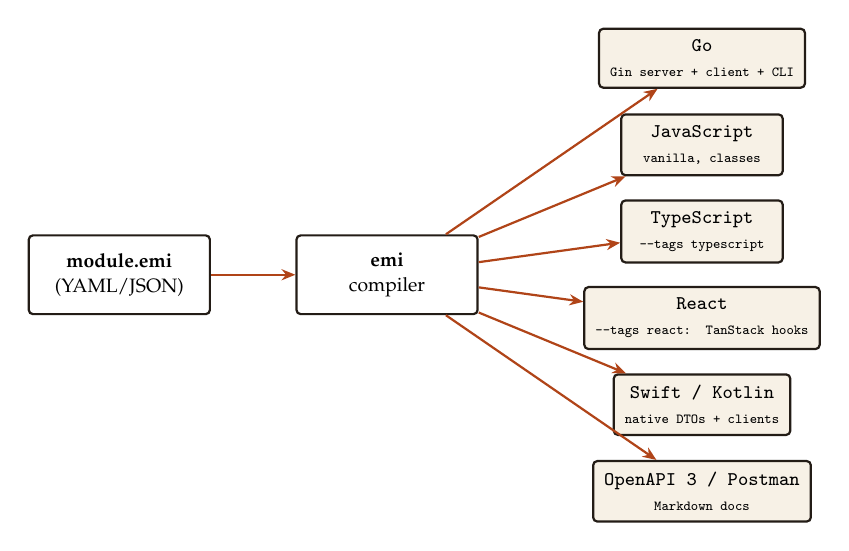
\begin{tikzpicture}[>=Stealth, node distance=1.1cm and 3.2cm]

  \node[src] (src) at (0,2.75) {module.emi\\[1pt]\normalfont\scriptsize(YAML/JSON)};
  \node[src] (compiler) at (3.4,2.75) {emi\\[1pt]\normalfont\scriptsize compiler};

  \node[ent] (go)     at (7.4,5.5) {Go\\[1pt]\tiny Gin server + client + CLI};
  \node[ent] (js)     at (7.4,4.4) {JavaScript\\[1pt]\tiny vanilla, classes};
  \node[ent] (ts)     at (7.4,3.3) {TypeScript\\[1pt]\tiny --tags typescript};
  \node[ent] (react)  at (7.4,2.2) {React\\[1pt]\tiny --tags react: TanStack hooks};
  \node[ent] (mobile) at (7.4,1.1) {Swift / Kotlin\\[1pt]\tiny native DTOs + clients};
  \node[ent] (docs)   at (7.4,0)   {OpenAPI 3 / Postman\\[1pt]\tiny Markdown docs};

  \draw[fk] (src) -- (compiler);
  \draw[fk] (compiler) -- (go);
  \draw[fk] (compiler) -- (js);
  \draw[fk] (compiler) -- (ts);
  \draw[fk] (compiler) -- (react);
  \draw[fk] (compiler) -- (mobile);
  \draw[fk] (compiler) -- (docs);

\end{tikzpicture}
\end{center}

\phantomsection\label{fig:pipeline}
\begin{center}
\begin{minipage}{0.94\linewidth}
\small\textbf{Fig.~1 --- The compilation pipeline.} One target-agnostic
definition, many sub-compilers, each reading the same document. The CLI
mirrors this diagram directly --- \texttt{emi go}, \texttt{emi js},
\texttt{emi swift}, \texttt{emi kotlin}, \texttt{emi openapi} --- and
\texttt{--tags} (\texttt{react}, \texttt{nestjs}, \texttt{typescript})
layer presentation choices onto a target's output without the definition
ever mentioning them. Because the compiler itself is written in Go and
also builds to \texttt{GOOS=js GOARCH=wasm}, the exact same compiler that
produces this fan-out also runs client-side in a browser tab --- no
server, no install (\S\ref{sec:in-browser}, and the
\href{https://torabian.github.io/emi/playground}{live playground}).
\end{minipage}
\end{center}

\begin{multicols}{2}
\raggedcolumns

\section{Go Compiler Features}
\label{sec:go-compiler-features}

The Go compiler is the only Emi target that generates a full server, not
just a client for one --- so this section tours what it adds on top of
the shared DTO/action codegen already covered above: database-backed
entities, typed relations with real migratable \href{https://gorm.io}{gorm}
associations, and the create/update actions generated for every entity.
Each part below shows a small sample of the Go code the compiler actually
emits.

\subsection{Entities}
\label{sec:go-entities}

An entity is a database-backed structure: its fields become both a Go
struct and database columns, migrated with \href{https://gorm.io}{gorm}.
Declared in a module's \texttt{entities:} list, right next to
\texttt{dtos:}/\texttt{actions:}:

\begin{lstlisting}
entities:
  - name: entity1
    table: entity1_table
    description: Exercises every supported field type.
    fields:
      - name: title
        type: string
\end{lstlisting}

\texttt{name} becomes the Go struct name (always upper-cased with
\texttt{Entity} appended --- \texttt{Entity1Entity}); \texttt{table}
overrides gorm's default pluralized/snake\_cased table name.

\subsubsection{Two fields every entity gets for free}
\begin{lstlisting}
type Entity1Entity struct {
  Id    int64  `gorm:"primaryKey;autoIncrement" json:"-"`
  UniqueId string `gorm:"type:uuid;default:gen_random_uuid();unique"
                    json:"uniqueId"`
  Title string `json:"title"`
}
\end{lstlisting}
\textbf{\texttt{Id}} is the real gorm primary key --- a plain
auto-incrementing integer, never exposed over JSON/CLI, so joins and
foreign keys can use a small integer instead of a UUID (smaller indexes,
faster joins). \textbf{\texttt{UniqueId}} is the public identifier every
API/CLI surface actually works with: a UUID generated natively by
Postgres itself (\texttt{gen\_random\_uuid()}, built into Postgres 13+)
via a column default, not application code. Both are prepended once, in
\texttt{EntityDefaultFields} (\texttt{lib/golang/go-entity-default-\allowbreak
fields.go}), before the struct generator, the update-input builder, and
the gorm-tag pass all run --- every consumer sees them as ordinary
declared fields.

\end{multicols}

\subsubsection{Field types on gorm}
\label{sec:go-gorm-types}
{\small
\begin{tabular}{@{}p{0.22\linewidth}p{0.74\linewidth}@{}}
\toprule
\textbf{Field type} & \textbf{Gorm tag} \\
\midrule
scalar (\texttt{string}, \texttt{int}, \ldots) & none --- gorm maps it directly \\
\texttt{enum}/\texttt{enum?} & none --- already a plain \texttt{string}/\texttt{Nullable[string]} \\
\texttt{object}/\texttt{object?} & \texttt{embedded} (inlined as columns) \\
\texttt{map}, \texttt{slice} (non-nullable) & \texttt{serializer:json} \\
\texttt{map?}, \texttt{slice?} & none --- \texttt{Nullable[T]} already implements \texttt{Value()}/\texttt{Scan()} \\
\texttt{complex} & none --- the type implements gorm's interfaces itself \\
\texttt{array}/\texttt{collection}/\texttt{one} & see relations, \S\ref{sec:go-relations} \\
\bottomrule
\end{tabular}
}

\begin{multicols}{2}
\raggedcolumns
An explicit \texttt{tags: \{ gorm: ... \}} on a field always wins over
these defaults. A \texttt{complex} field used on an entity must implement
\texttt{driver.Valuer}/\texttt{sql.Scanner} itself --- the generator has
no way to guess how to persist a hand-written type.

Every entity file ends with a small, separate template
(\texttt{go-entity.tpl}) whose output is appended \emph{after} the
generated struct --- currently a \texttt{TableName()} override wired to
\texttt{table:}, and the place to extend if a project wants something
appended to every generated entity file.

\subsubsection{Browsing: JSON Logic filters}
An entity with browsing enabled also gets a generated
\texttt{\{Entity\}BrowseFn} and a \texttt{GET /entity1/browse} action,
exposing five query params: \texttt{filter}, \texttt{sort},
\texttt{startIndex}, \texttt{itemsPerPage}, \texttt{cursor}.
\texttt{filter} is a \href{https://jsonlogic.com}{JSON Logic} expression,
transpiled straight to SQL by \texttt{emigorm.ApplyQueryFilter} --- never
string-concatenated, and never a filter language Emi invented itself:
\begin{lstlisting}
GET /entity1/browse?filter={"==":[{"var":"title"},"hello"]}
GET /entity1/browse?filter={"and":[
  {">":[{"var":"age"},18]},
  {"contains":[{"var":"title"},"draft"]}
]}
\end{lstlisting}
Every standard JSON Logic operator works (\texttt{==}, \texttt{!=},
\texttt{>}, \texttt{<}, \texttt{and}, \texttt{or}, \texttt{in}, \ldots)
plus one Emi adds itself: \texttt{contains} --- a case-insensitive
substring match (\texttt{::text ILIKE '\%...\%'}), the one operator
plain JSON Logic has no native equivalent for.

Sort and paging are the plain, non-JSON-Logic half:
\texttt{sort=createdAt desc} (empty defaults to \texttt{id asc}, needed
for keyset paging to stay correct), and either offset paging
(\texttt{startIndex}/\texttt{itemsPerPage}) or cursor paging
(\texttt{cursor}, echoing the response's own cursor field back on the
next call --- \texttt{cursor=id(42)}).

\begin{pullquote}
\texttt{filter} is the only \emph{user}-controlled half of a Browse
query. A handler's own tenant/workspace isolation goes through the
separate \texttt{emigorm.ApplyQueryScope} (a raw SQL fragment the
handler itself writes, applied unconditionally) --- \texttt{filter} has
no way to see or override it.
\end{pullquote}

\subsection{Writing a complex type}
\label{sec:go-complex}
A \texttt{complex: Money} field (\S\ref{sec:complex-types}) needs a real
Go type at the declared \texttt{location}/\texttt{namespace} --- nothing
more, to just carry the value through a DTO or action. Persisting it on
an \texttt{entity} is a separate, opt-in step: gorm has no idea how to
store an arbitrary hand-written struct, so the type has to say so itself.

\subsubsection{Nullability: no wrapper, no pointer}
A \texttt{complex} field is the one place Go's nullable-field convention
doesn't apply. Every other nullable field type gets wrapped in
\texttt{emigo.Nullable[T]} (\S\ref{sec:go-gorm-types}); a complex field
never does, whether the field is declared \texttt{complex} or (the
JS-only variant) \texttt{complex?} --- both compile to the exact same
plain \texttt{Money} value in Go, because a complex value has no
wire-level nullability of its own as far as the Go compiler is concerned.
\texttt{complex?} exists purely so the JS/TS compiler can tell ``always
instantiate'' apart from ``allow \texttt{undefined}/\texttt{null} on the
setter''; every other backend, Go included, treats the two identically.

The one place a complex field \emph{does} become a pointer is inside the
generated \texttt{\{Entity\}UpdateInput} struct (\S\ref{sec:go-actions}):
since there's no \texttt{Nullable[T]} counterpart for a hand-written
type, the update-input builder falls back to a plain \texttt{*Money},
where \texttt{nil} means ``untouched'' --- the same ``was this field
mentioned at all'' signal every other field gets from
\texttt{Nullable[T]}'s own \texttt{IsSet()}, just spelled with a raw
pointer instead of a generic wrapper.

\subsubsection{Persisting to one column}
Implementing \texttt{database/sql/driver.Valuer} and \texttt{sql.Scanner}
stores the whole value as a single column:
\begin{lstlisting}
type Money struct {
  Cents int64
}

func (m Money) Value() (driver.Value, error) {
  return m.Cents, nil
}

func (m *Money) Scan(value interface{}) error {
  switch v := value.(type) {
  case int64:
    m.Cents = v
  case []byte:
    cents, err := strconv.ParseInt(string(v), 10, 64)
    if err != nil {
      return err
    }
    m.Cents = cents
  }
  return nil
}
\end{lstlisting}
A real complex type is expected to implement whatever interfaces its own
storage needs --- \texttt{MarshalText}/\texttt{UnmarshalText} too, if it
should also cast cleanly from a CLI string argument, the same way
fireback's own complex types (e.g.\ \texttt{XDate}) do.

\subsubsection{Persisting across multiple columns}
Valuer/Scanner is a single-column round trip; not every complex type fits
one column. Skip both interfaces and gorm falls back to walking the
struct like it does for an \texttt{object}/\texttt{object?} field
(\S\ref{sec:go-gorm-types}) --- each exported field becomes its own column:
\begin{lstlisting}
type Address struct {
  Street string `gorm:"column:addr_street"`
  City   string `gorm:"column:addr_city"`
  Zip    string `gorm:"column:addr_zip"`
}
\end{lstlisting}
No \texttt{Value()}/\texttt{Scan()} at all here --- the struct is plain
data, and gorm's own reflection spreads it across \texttt{addr\_street},
\texttt{addr\_city}, \texttt{addr\_zip} exactly as it would for any
embedded struct. Pick single-column when the type has one natural
serialized form (money as cents, a date as text); pick multi-column when
it's naturally shaped as several fields side by side.

\subsection{Relations: array, collection, one}
\label{sec:go-relations}

A dto's \texttt{one}/\texttt{collection} field just needs a Go type to
hold data. An entity's relation field needs that \emph{and} a real,
migratable gorm association --- and the two shapes are incompatible in a
way that isn't obvious up front. \texttt{array}/\texttt{collection}/
\texttt{one} normally render as \texttt{emigo.Array[T]}/
\texttt{Collection[T]}/\texttt{One[T]} --- PATCH-payload wrapper types
carrying an \texttt{Operation} (\texttt{replace}/\texttt{append}/
\texttt{select}) --- the right shape for an API, but not one gorm can
migrate (verified directly against \texttt{gorm.io/gorm/schema.Parse}).

So an entity keeps the DTO field as-is (still the only public JSON/CLI
surface) tagged \texttt{gorm:"-"}, and generates a hidden sibling field
that \emph{is} a real gorm association:

\begin{lstlisting}
Items    emigo.Array[Entity1EntityItems] `gorm:"-" json:"items"`
Owner    emigo.One[Entity2Entity]        `gorm:"-" json:"owner"`

ItemsRow []*Entity1EntityItems `gorm:"foreignKey:LinkerId;references:Id;
                                 constraint:OnDelete:CASCADE" json:"-"`
OwnerId  int64          `gorm:"index" json:"-"`
OwnerRow *Entity2Entity `gorm:"foreignKey:OwnerId;references:Id" json:"-"`
\end{lstlisting}
The \texttt{\{field\}Row}/\texttt{\{field\}Id} siblings are purely a
persistence concern (\texttt{json:"-"}); whatever writes to the database
(\S\ref{sec:go-actions}) keeps the DTO field and its sibling in sync.

\begin{sidebar}{The three relation kinds}
\textbf{array} --- has-many, owned composition. Nested \texttt{fields:}
become a child struct with its own \texttt{Id}/\texttt{UniqueId} plus a
\texttt{LinkerId} FK back to the parent.

\textbf{collection} --- many-to-many, backed by a join table named
\texttt{\{entity\}\_\{field\}} (e.g.\ \texttt{entity1\_items3}).

\textbf{one} --- belongs-to: a foreign-key column on \emph{this} entity,
named \texttt{\{field\}Id}, referencing the target's \texttt{Id}.
\end{sidebar}

\textbf{Why \texttt{Id} and not \texttt{UniqueId}}: every
\texttt{foreignKey}/\allowbreak\texttt{references} tag joins on the small integer
\texttt{Id}, keeping indexes smaller and joins faster, even though
\texttt{UniqueId} is the only identity an API caller ever actually has.
Since gorm's \texttt{Save()} decides insert-vs-update purely from whether
\texttt{Id} is already populated, and a caller only ever knows
\texttt{UniqueId}, the reconcile helpers (\S\ref{sec:go-actions}) resolve
an incoming item's real \texttt{Id} by matching \texttt{UniqueId} first.

\subsubsection{Relations nested inside object containers}
A relation doesn't have to sit directly on the entity --- it can live
inside an \texttt{object} (or \texttt{object?}) field, any depth deep.
Gorm's own embedding correctly walks an arbitrarily deep \texttt{embedded}
chain and still recognizes the association, keyed by its bare field name
rather than the full nested path (verified against
\texttt{gorm.io/gorm/schema.Parse} and a real database run) --- provided
the nested child struct is named with the same accumulating prefix the
struct generator uses for the container itself, and
\texttt{\{Entity\}CreateFn}/\texttt{UpdateFn} recurse into
\texttt{object}/\texttt{object?} containers to find relations at any
depth. \texttt{object?} specifically needs its own fix: it renders as
\texttt{emigo.Nullable[T]}, and gorm's embedding only ever sees the
wrapper's own unexported fields, never \texttt{T}'s --- so it gets the
same \texttt{\{field\}Row *T} hidden-sibling treatment a relation does,
even for a field with no relation in it at all.

\begin{pullquote}
Known limitations: a relation declared on an array item itself (rather
than on the entity or one of its object containers) isn't picked up ---
each array item is still persisted as one flat unit via \texttt{Save()}.
Cross-module targets (\texttt{module:} on a relation field) aren't
accounted for in the FK/table naming yet.
\end{pullquote}

\sectiontheme{goblue}
\subsection{Create \& Update Actions}
\label{sec:go-actions}

Every entity gets two generated functions --- \texttt{\{Entity\}CreateFn}
and \texttt{\{Entity\}UpdateFn} --- plus a small actions bundle wiring
them up as the defaults, mirroring the pattern
\href{https://github.com/torabian/fireback}{fireback} uses.

\subsubsection{Request body formats}
Every generated Go action --- Create/Update included --- reads its body
through \texttt{emigo.BindGinRequestBody}, which picks the decoder from
the request's own \texttt{Content-Type} rather than assuming JSON:
\begin{itemize}[leftmargin=1.1em,itemsep=2pt,topsep=2pt]
  \item \texttt{application/json} --- the default, and what every
    generated client sends.
  \item \texttt{application/yaml}/\texttt{x-yaml}/\texttt{text/yaml}
    --- the same struct, from YAML.
  \item \texttt{application/xml}/\texttt{text/xml}.
  \item \texttt{multipart/form-data} --- each non-file field round-trips
    through JSON into the struct; each uploaded file becomes a
    \texttt{BindMultipartFile} (\texttt{filename}/\texttt{mime}/
    \texttt{data}), unless the host app registers its own
    \texttt{ConvertMultipartFile} (fireback, for instance, turns one into
    an \texttt{XFile}).
  \item \texttt{application/x-www-form-urlencoded} --- a plain HTML
    \texttt{<form method="post">} postback works unmodified, no
    JavaScript or fetch call required: the browser's own form submission
    already sends this content type, and every field lands in the same
    generated struct a JSON body would.
\end{itemize}
Only \texttt{POST}/\texttt{PATCH}/\texttt{PUT} read a body at all --- a
no-op for every other method, matching plain HTTP. The response side
mirrors this: \texttt{RenderGinResult} content-negotiates off the
request's \texttt{Accept} header (JSON, YAML, TOML, or CSV; JSON when
unset or unrecognized), so a caller gets the format it asked for without
the handler itself knowing or caring which one that is.

\subsubsection{The update input: optional, all the way down}
A struct-based \texttt{gorm.Updates()} call silently drops zero-valued
fields, so it can't tell ``the caller didn't mention this field'' apart
from ``the caller explicitly set it to zero.'' Every entity therefore
gets a second generated type, \texttt{\{Entity\}UpdateInput}, where
\emph{every} field --- even a plain, always-present scalar on the entity
itself --- is wrapped optional:
\begin{lstlisting}
type Entity1EntityUpdateInput struct {
  Title  emigo.Nullable[string] `json:"title"`
  Items  emigo.ArrayNullable[Entity1EntityItems] `json:"items"`
  Owner  emigo.OneNullable[Entity2Entity]         `json:"owner"`
  Complex1 *Money                                 `json:"complex1"`
}
\end{lstlisting}
\texttt{id}/\texttt{uniqueId} are left out entirely --- immutable
identity, not something an update patches. A \texttt{complex} field (no
\texttt{?} counterpart exists) becomes a plain pointer instead;
\texttt{nil} means untouched. Critically, \texttt{array}/
\texttt{collection}/\texttt{one} fields reuse the \emph{real} row/target
type directly, not a second, separately-optional clone --- only whether
the field itself was touched (\texttt{IsSet()}) is optional; an item
included in a replace/append batch still has to be given in full, exactly
like Create, because the reconcile helpers persist each item with a plain
\texttt{Save()} that writes every field.

\subsubsection{The reconcile helpers (\texttt{emigorm})}
Gorm's own \texttt{Association().Replace()} was verified \textbf{unreliable}
for a has-many \texttt{array} relation: an incoming item whose primary key
already exists silently keeps its \emph{old} content, and items dropped
from the list are never deleted --- just orphaned. So
\texttt{github.com/torabian/emi/emigorm} (kept out of the wasm-safe
\texttt{emigo} core since it depends on \texttt{gorm.io/gorm}) provides
three reconcile functions instead:

\begin{sidebar}{One reconciler per relation kind}
\textbf{ReconcileHasMany} (\texttt{array}) --- diffs existing children
against the incoming list by \texttt{UniqueId}, hard-deletes any row
missing from a \texttt{"replace"} batch, \texttt{Save()}s every incoming
item. \texttt{"append"} skips the diff/delete step.

\textbf{ReconcileManyToMany} (\texttt{collection}) --- gorm's Association
API \emph{is} reliable here, so this upserts inline target values first,
then delegates to \texttt{Association().Replace()}/\texttt{.Append()}.

\textbf{ReconcileOne} (\texttt{one}) --- \texttt{"select"} resolves an
existing target's \texttt{Id} from its \texttt{UniqueId} and leaves it
untouched; anything else upserts the inline value.
\end{sidebar}

All three resolve an incoming item's real \texttt{Id} by matching
\texttt{UniqueId} against an existing row \emph{before} calling
\texttt{Save()} --- otherwise every ``update'' would silently insert a
duplicate.

\subsubsection{Testing}
Every relation is verified two ways: \textbf{structurally}, with no
database at all, via \texttt{gorm.io/gorm/schema.Parse} (confirms every
\texttt{has\_many}/\texttt{many\_to\_many}/\texttt{belongs\_to} resolves
correctly in milliseconds); and \textbf{end to end against real
Postgres} (\texttt{examples/emi-entity/sdk/*\_test.go}) --- cascading
create, partial update, array replace-with-orphan-deletion, collection
append, and one re-select are all covered. Since \texttt{UniqueId}'s
column default is Postgres-specific, the live tests need a real Postgres
instance (\texttt{make entity-db-up}); MySQL is wired up too but expected
to fail on the same \texttt{gen\_random\_uuid()} default --- an accepted
tradeoff, not something actively kept green.

\section{Legal Notices: Permissions \& Events}
\label{sec:permissions-events}

\subsection{Permissions: a compiled tree}
A module can declare a \texttt{permissions:} tree --- nested access
control permissions the module contributes. Each node has a \texttt{key}
(its slug) and a \texttt{name} (used to name the generated identifier,
e.g.\ \texttt{name: managePosts} $\to$ \texttt{ManagePostsPermission}).
The full identifier is either set explicitly via \texttt{fullKey:} or
computed as \texttt{\{parent.fullKey\}.\{key\}} during preprocessing; a
node that groups children and left its key to be derived gets a trailing
\texttt{.*} (e.g.\ \texttt{post.*}), signaling it covers itself and
everything below.

\begin{lstlisting}
permissions:
  - key: post
    name: managePosts
    children:
      - key: create
        name: createPost
      - key: publish
        name: publishPost
\end{lstlisting}

Compiling this (Go target) produces one exported var \textbf{per root
permission} --- not one var wrapping the whole forest, and no separate
flat constant per node either. Each var is a fully typed, nested struct:
every node embeds \texttt{emigo.Permission} (promoting its own
\texttt{Key}) and has one field per child, so an editor autocompletes
straight down it with zero risk of a typo'd key only failing at runtime:
\begin{lstlisting}
var ManagePostsPermission = struct {
  emigo.Permission
  CreatePost  emigo.Permission
  PublishPost emigo.Permission
}{ /* ... */ }

var ManagePostsPermissionList = []emigo.Permission{
  ManagePostsPermission.Permission,
  ManagePostsPermission.CreatePost,
  ManagePostsPermission.PublishPost,
}
\end{lstlisting}
\texttt{<Name>PermissionList} sits alongside every root, built by
referencing the root var's own fields rather than re-declaring separate
literals, so it can never drift out of sync with it --- one list per
root, not one combined list a caller has to filter back down. The JS/TS
compiler mirrors this shape as a \texttt{const ... as const} object (or
\texttt{Object.freeze(...)} without \texttt{--tags typescript}) instead of
a Go struct, with the same one-const-per-root, \texttt{<Name>PermissionList}
convention.

\subsection{Events: flat facts, typed payloads}
A module can declare an \texttt{events:} list --- flat, unlike
\texttt{permissions:}, since an event is a single fact (``a post got
published''), not a tree. Each event has a \texttt{key} (its wire name),
optional localized \texttt{name}/\texttt{description}, a \texttt{payload},
and \texttt{permissions} describing who's allowed to know it happened ---
a list of \texttt{with} blocks, OR'd together, each entry's \texttt{with}
list AND'd (\texttt{[\{with: [A,B]\}, \{with: [C,D]\}]} means
\texttt{(A and B) or (C and D)}).

\begin{lstlisting}
events:
  - key: postPublished
    permissions:
      - with: ["post.publish"]
      - with: ["post.*"]
    payload:
      fields:
        - {name: postId, type: string}
  - key: commentAdded
    payload:
      dto: CommentDto
  - key: postArchived
\end{lstlisting}

Three events, three payload shapes: \texttt{postPublished} declares
\texttt{fields} inline, compiled into a dedicated
\texttt{PostPublishedEventPayload} struct exactly like an action's
request body, complete with CLI flags; \texttt{commentAdded} points
\texttt{dto:} at an existing dto, so its payload type is a plain alias,
not a new struct; \texttt{postArchived} declares no payload at all, so
its payload type aliases straight to \texttt{interface\{\}}. One exported
var is generated per event (PascalCase, trailing \texttt{Event}), always
paired with a \texttt{<EventName>Payload} type and a
\texttt{New<EventName>(payload)} constructor, and every var is collected
into \texttt{AllEventsList} for anything that wants to walk the whole
catalog. The compiler rejects the module outright if two differently
spelled keys (\texttt{postPublished} vs.\ \texttt{post\_published})
would normalize to the same generated identifier, rather than letting one
silently shadow the other.

\section{The Style Section: JavaScript/TypeScript}
\label{sec:js-compiler}

JavaScript gets special focus in Emi, because nearly everything eventually
has to be consumed by a JS environment. The JS output is real, runnable
JavaScript --- no transpile step required --- while \texttt{--tags
typescript} produces high-coverage \texttt{.ts} with, Emi's docs claim,
some of the highest-quality TypeScript output among competing generators.
\texttt{--tags react} layers on TanStack React Query hooks plus an
internal \texttt{useSse} and \texttt{useWebSocketX}; \texttt{--tags
nestjs} emits decorators that make request, headers and query params
portable straight into Nest.js handlers with no extra code.

\subsection{Auto-init: every field guaranteed to exist}
When an action returns a class instance, \emph{every} non-nullable field
--- including nested objects, arrays, and child DTOs --- is guaranteed to
exist. Writing this by hand is a hassle and easy to get subtly wrong;
Emi generates it from the definition alone:
\begin{lstlisting}
fields:
  - name: object1
    type: object
    fields:
      - name: contacts
        type: array
        fields:
          - name: email
            type: string
            default: emi-compiler@emi-compiler.com
          - name: phone
            type: string?
\end{lstlisting}
produces a class whose \texttt{object1} field is \emph{always} an
instance of a nested \texttt{AutoInitClassDto.Object1} class, never
\texttt{undefined} --- the code stops sprinkling \texttt{?.}, \texttt{??},
and \texttt{typeof x === 'string'} defensively, because the class already
did the guarding.

\subsection{Ergonomics every generated class ships with}
\begin{itemize}[leftmargin=1.1em,itemsep=2pt,topsep=2pt]
  \item \texttt{from()} --- full object constructor; \texttt{with()} ---
        partial, deeply-typed via \texttt{PartialDeep}.
  \item \texttt{copyWith()}, \texttt{clone()}, a correct \texttt{toJSON()}
        that sees the private fields (plain \texttt{JSON.stringify}
        otherwise can't --- the fields are genuinely private).
  \item A static \texttt{Fields} map (e.g.\ \texttt{Fields.date === "date"})
        for safe, refactor-proof path access instead of a hardcoded string
        literal.
\end{itemize}

\subsection{The Headers class}
HTTP request/response headers are a key/value definition; Emi generates a
class extending the standard \texttt{Headers} with typed
\texttt{getX()}/\texttt{setX()} accessors that coerce values on the way
out:
\begin{lstlisting}
- {name: accept-language, type: string}
- {name: cache-time,      type: int64}
\end{lstlisting}
\begin{lstlisting}
export class SampleHeaders extends Headers {
  getAcceptLanguage() { return this.#getTyped('accept-language', 'string|null'); }
  setCacheTime(value: number|null) {
    if (value !== null) this.set('cache-time', value);
    return this;
  }
}
\end{lstlisting}
\texttt{.get()} on the plain \texttt{Headers} base still returns the raw
string --- the typed accessors are additive, not a replacement.

\begin{pullquote}
Header/query-param typing at this level --- including \emph{nested} query
params rendered as typed accessors --- is a feature Emi's own docs single
out as unique among the generators it's compared against.
\end{pullquote}

\sectiontheme{jsyellow}
\section{JSON Schema on the JavaScript Side}
\label{sec:json-schema}

Every JS/TS dto already has a field-plan tree the compiler walks to render
a form (\S\ref{sec:js-compiler}); \texttt{lib/formgen} walks that same
tree a second way, into a renderer-agnostic JSON Schema instead of a
bespoke component. There are two ways to get one out.

\subsection{Two ways to get a schema}
\textbf{Per-dto, standalone} --- \texttt{emi js:rjsf} takes a single
\texttt{emi: dto} definition and writes two files: the schema itself, and
a thin wrapper component around \href{https://rjsf-team.github.io/react-jsonschema-form/}{react-jsonschema-form}
(RJSF) that renders it:
\begin{lstlisting}
emi js:rjsf --path address.emi.yml --output ./out
# ./out/AddressDto.schema.json
# ./out/AddressDtoForm.tsx
\end{lstlisting}

\textbf{Embedded on the class} --- \texttt{--tags json-schema} on a full
module compile instead attaches every generated dto/action-request/
action-response class's schema directly to itself, as
\texttt{static JsonSchema = \{...\}} (off by default --- it's extra
bytes most consumers don't need):
\begin{lstlisting}
emi js --path module.emi.yml --output ./out --tags json-schema,typescript
\end{lstlisting}
Both read the exact same \texttt{BuildJSONSchema} tree walk
(\texttt{lib/formgen/jsonschema.go}), so the shape of the schema itself
never depends on which of the two you use --- only where it ends up.

\subsection{A minimal example}
\begin{lstlisting}
name: address
fields:
  - name: street
    type: string
    description: Street and number
  - name: unit
    type: string?
  - name: kind
    type: enum
    enum:
      - key: home
        description: Home address
      - key: work
  - name: manager
    type: one
    target: employee
\end{lstlisting}
compiles (\texttt{emi js:rjsf}) to:
\begin{lstlisting}
{
  "type": "object",
  "title": "AddressDto",
  "properties": {
    "street": { "type": "string", "title": "Street", "description": "Street and number" },
    "unit":   { "type": "string", "title": "Unit" },
    "kind":   { "type": "string", "title": "Kind", "oneOf": [
      { "const": "home", "title": "Home address" },
      { "const": "work", "title": "work" }
    ]},
    "manager": { "title": "Manager" }
  },
  "required": ["street", "kind", "manager"]
}
\end{lstlisting}

\begin{sidebar}{Two things worth noticing}
\texttt{unit} is missing from \texttt{required} --- the trailing
\texttt{?} is the only thing that removes a field from it, independent
of the field's own type or widget. And \texttt{manager} --- a
\texttt{one} relation, so genuinely unconstrained (\texttt{\{title:
"Manager"\}}, no \texttt{type}) --- is still \emph{in} \texttt{required},
because it isn't nullable: \texttt{required} tracks nullability alone,
not whether the schema actually constrains the value. RJSF only checks
the key is present, so an empty object still satisfies it.
\end{sidebar}

An \texttt{enum} option's human label comes from its \texttt{description}
(falling back to the raw key, as \texttt{work} does above); \texttt{one}/
\texttt{collection} relation fields and \texttt{any}/\texttt{complex}
fields both resolve to an unconstrained \texttt{\{\}} on purpose --- the
schema compiler was never given the target entity's own fields (a
relation) or has no fixed shape to begin with (\texttt{any}), so it
leaves the value alone rather than guessing, deliberately mirroring the
same ``leave it to a custom field on the renderer side'' choice
\S\ref{sec:js-complex} makes for a hand-written complex type.

\subsection{Using it in the front end}
The RJSF wrapper is a controlled component --- \texttt{value}/
\texttt{onChange}, the same convention every other generated form
component in Emi uses --- so a consuming app drops it in with zero
manual field wiring, validation included:
\begin{lstlisting}
import AddressDtoForm from "./out/AddressDtoForm";

function EditAddress() {
  const [value, setValue] = useState<Partial<AddressDto>>({});
  return <AddressDtoForm value={value} onChange={setValue} />;
}
\end{lstlisting}
Under the hood that wrapper is nothing more than the schema plus RJSF's
own \texttt{<Form>} and \texttt{@rjsf/validator-ajv8} --- swap either
import and the same generated \texttt{.schema.json} still works, since
nothing about it is RJSF-specific.

The embedded \texttt{static JsonSchema} form exists for the opposite
case: an app that isn't using RJSF at all still gets a real JSON Schema
for free on every generated class, to hand to a different schema-driven
renderer, validate a payload with a bare \texttt{ajv} instance before a
submit, or drive a headless dynamic-form engine --- all without a second
compile step or a hand-maintained schema that can drift from the dto.

\begin{pullquote}
Both paths are opt-in and additive: no code Emi already generates for a
dto changes shape because a schema exists alongside it, and skipping
both (the default) costs nothing --- no \texttt{formgen} import ends up
in the output at all.
\end{pullquote}

\section{Reactive: WebSocket \& SSE}
\label{sec:reactive}

Marking an action \texttt{method: reactive} tells Emi the endpoint is a
WebSocket, full-duplex channel. The JS compiler generates a
\texttt{WebSocketX} class --- the base every reactive action's generated
code sits on top of --- which extends the standard \texttt{WebSocket}
with the exception that \texttt{message} and \texttt{send} are overridden
to accept generic types, and the constructor takes a factory for message
creation when working with JSON messages. Other generators (React, for
instance) wrap the instance rather than replacing it, layering a
\texttt{useWebSocketX} hook on top.

\begin{lstlisting}
actions:
  - name: userStream
    url: ws://localhost:8081
    method: reactive
    in:
      fields:
        - {name: min,   type: int}
        - {name: max,   type: int}
        - {name: count, type: int}
    out:
      fields:
        - {name: number, type: int}
\end{lstlisting}

produces a complete typed request/response pair plus an action wrapper:

\begin{lstlisting}
export class UserStreamAction {
  static URL = "ws://localhost:8081";
  static Method = "REACTIVE";
  static Create = (overrideUrl?, qs?, options) => {
    const Cls = options?.SocketClass ??
      WebSocketX<UserStreamActionReq, UserStreamActionRes>;
    return new Cls(url, undefined, {
      MessageFactoryClass: UserStreamActionRes,
    });
  };
}
\end{lstlisting}

The generated request (\texttt{UserStreamActionReq}) and response
(\texttt{UserStreamActionRes}) classes are ordinary Emi DTO classes ---
same private fields, typed getters/setters, and auto-init guarantees as
any other generated class (\S\ref{sec:js-compiler}); the only thing
\texttt{reactive} changes is the transport they travel over. The
generated JavaScript works in both Node.js and browser environments,
though the client side is the primary focus.

\begin{pullquote}
SSE gets the same treatment as WebSocket in spirit: a plain \texttt{get}
action whose response streams chunked messages compiles to typed
messages on the client, and \texttt{--tags react} adds a matching
\texttt{useSse} hook right alongside \texttt{useWebSocketX}.
\end{pullquote}

\section{Foreign Desk: Swift \& Kotlin Clients}
\label{sec:swift-kotlin}

\subsection{Swift}
The Swift compiler generates plain \texttt{Foundation}-based code (falling
back to \texttt{FoundationNetworking} on Linux) --- no third-party
dependency pulled in. It produces type-safe request/response objects and
an action wrapper per action, mirroring every other Emi compiler:
\begin{lstlisting}
emi swift --path module.yaml --output ./Sources/Generated
\end{lstlisting}
\texttt{emi swift:dto} and \texttt{emi swift:headers} generate just the
DTOs or just the headers, when the full compiler's output isn't needed.
Each action carries its own metadata struct (name, URL, method) and a
strongly typed response, so calling code never hardcodes a route or
guesses a response shape:
\begin{lstlisting}
struct GetSinglePostActionMeta {
    let name: String = "GetSinglePostAction"
    let url: String = "/posts/:id"
    let method: String = "Get"
}
struct GetSinglePostActionResponse {
    let statusCode: Int
    let headers: [String: String]
    let payload: Data?
}
\end{lstlisting}

\subsection{Kotlin}
The Kotlin compiler targets Android and JVM projects from the same
definitions, using \href{https://github.com/Kotlin/kotlinx.serialization}{kotlinx.serialization}
for JSON and \href{https://square.github.io/okhttp/}{OkHttp} for
networking --- both need to be on the consuming project's classpath, and
nothing else does:
\begin{lstlisting}
emi kotlin --path module.yaml \
  --output ./src/main/kotlin/generated
\end{lstlisting}
One invocation compiles everything a module declares --- \texttt{dtos:},
\texttt{entities:} (each becomes a dto plus a set of CRUD actions), and
\texttt{actions:} --- into a flat directory of \texttt{.kt} files plus
shared runtime files. \texttt{emi kotlin:dto} and \texttt{emi
kotlin:headers} narrow the output the same way their Swift counterparts
do. \texttt{--pkg} sets the Kotlin \texttt{package} every generated file
is written under (default \texttt{unknownpackage}) --- it only matters
once more than one module compiles into the same project, so cross-module
dto/entity references resolve to the right package.

\begin{sidebar}{Shared shape across both compilers}
\begin{itemize}[leftmargin=1.1em,itemsep=1pt,topsep=2pt]
  \item \texttt{--path} / \texttt{--output} --- same convention as every
        Emi sub-compiler
  \item Without \texttt{--output}, generated virtual files print as JSON
        to the terminal for inspection before anything touches disk
  \item \texttt{--tags} --- comma-separated compile features, same
        mechanism as the Go and JS compilers
\end{itemize}
\end{sidebar}

\section{Additional Language Targets}
\label{sec:additional-targets}

Every remaining client target takes the same \texttt{.emi.yml} through
its own sub-compiler, with the same \texttt{--path}/\texttt{--output}
pair every other Emi compiler already uses. Each one below is
client-only --- no server, no CLI, no entity/gorm persistence --- and
most share the same two housekeeping tags: \texttt{no-sdk} (skip
embedding the runtime files) and \texttt{no-pkg} (skip the
language-native package manifest --- \texttt{requirements.txt},
\texttt{pom.xml}, \texttt{.csproj}, \texttt{composer.json},
\texttt{pubspec.yaml}, \texttt{README.md}, depending on the target).

\subsection{Python}
\texttt{dataclasses}-based DTOs and an \texttt{httpx} client, synchronous
by default:
\begin{lstlisting}
emi python --path module.emi.yml --output ./out/python
emi python --path module.emi.yml --output ./out/python --tags async
\end{lstlisting}
\texttt{--tags async} swaps every generated client function to
\texttt{async def}, backed by \texttt{httpx.AsyncClient}, instead.

\subsection{Dart}
DTO classes with hand-generated \texttt{toJson}/\texttt{fromJson} and a
\texttt{package:http} client:
\begin{lstlisting}
emi dart --path module.emi.yml --output ./out/dart
\end{lstlisting}

\subsection{C\#}
\texttt{System.Text.Json}-based DTOs and an \texttt{HttpClient} transport:
\begin{lstlisting}
emi csharp --path module.emi.yml --output ./out/csharp
\end{lstlisting}

\subsection{Java}
Jackson-based DTOs on top of \texttt{java.net.http.HttpClient}:
\begin{lstlisting}
emi java --path module.emi.yml --output ./out/java
\end{lstlisting}

\subsection{PHP}
Reflection-based DTO hydration and a \texttt{curl} HTTP transport:
\begin{lstlisting}
emi php --path module.emi.yml --output ./out/php
\end{lstlisting}

\subsection{C}
Vendored \texttt{cJSON} (de)serialization and \texttt{libcurl} transport
--- no nullable value types without pointers, a documented scope limit:
\begin{lstlisting}
emi c --path module.emi.yml --output ./out/c
\end{lstlisting}

\subsection{C++: generic and Unreal Engine}
One compiler, two dialects, picked with \texttt{--dialect} (or the
equivalent \texttt{--tags unreal}, handy when a caller is already
building a \texttt{--tags} list): portable ISO C++17 for desktop/ESP-IDF/
Arduino by default, or \texttt{USTRUCT}/\texttt{UPROPERTY} DTOs usable
from Blueprint when the Unreal dialect is selected.
\begin{lstlisting}
emi cpp --path module.emi.yml --output ./out/cpp                  # generic ISO C++17
emi cpp --path module.emi.yml --output ./out/cpp-unreal \
  --dialect unreal                                                # Unreal Engine
\end{lstlisting}

\begin{pullquote}
\texttt{--path}, \texttt{--output}, and \texttt{--tags} is the interface
every Emi compiler shares, this section's seven targets included --- run
\texttt{emi tags} at any time to print the full, current tag list for
every registered target, straight from the compiler's own source of
truth rather than a copy that can drift out of date here.
\end{pullquote}

\sectiontheme{rustaccent}
\section{Exports: Markdown, OpenAPI, Postman}
\label{sec:exports}

Three commands don't emit source code at all --- they \emph{describe} a
module in a standard interoperable format, reading the same definition
that produces the Go/Swift/Kotlin/JS clients, so none of them can drift
away from the real implementation.

\subsection{\texttt{emi md} --- Markdown docs}
The fastest way to get human-readable, always up to date documentation
for a module: a title, description, table of contents, and one section
per action listing method, URL, CLI name, and request/response fields.
\begin{lstlisting}
emi md --path module.yaml --output ./out
# ./out/postsModule.md
\end{lstlisting}
Output for a single-action module looks like:
\begin{lstlisting}
### `GetSinglePostAction`
| | |
|---|---|
| **Method** | `GET` |
| **URL** | `/posts/:id` |
| **CLI** | `get-single-post` |
#### Response
| Field | Type |
|---|---|
| `userId` | `int64` |
\end{lstlisting}
Committed next to the module, served in a docs site, or rendered straight
into a README.

\subsection{\texttt{emi openapi} --- OpenAPI 3}
A \emph{describer}, not a compiler: reads the definition, produces a
standard \href{https://spec.openapis.org/oas/v3.0.3}{OpenAPI 3} document
for Swagger UI, Redoc, code generators, or API gateways.
\begin{lstlisting}
emi openapi --path module.yaml --output ./out --json
# ./out/postsModule.openapi.yaml (+ .json)
\end{lstlisting}
Route parameter syntax is rewritten (\texttt{/posts/:id} becomes
\texttt{/posts/\{id\}}), path parameters are promoted, and Emi field
types map onto the correct OpenAPI \texttt{type}/\texttt{format} pairs
(e.g.\ \texttt{int64} $\to$ \texttt{type: integer, format: int64}).

\subsection{\texttt{emi postman} --- Postman v2.1 collection}
Every action becomes a Postman request with method, URL, and the standard
Emi headers pre-filled, ready to import and start hitting endpoints
immediately.
\begin{lstlisting}
emi postman --path module.yaml \
  --host localhost --port 8080 --output ./out
\end{lstlisting}
Host and port are emitted as Postman environment variables
(\texttt{\{\{HOST\}\}}, \texttt{\{\{PORT\}\}}) so switching between
local, staging and production is a matter of changing the active
environment, and the common Emi headers (\texttt{authorization},
\texttt{role-id}, \texttt{workspace-id}) are wired to
\texttt{\{\{AUTH\}\}}/\texttt{\{\{RID\}\}}/\texttt{\{\{WID\}\}}
variables, filled once and reused across every request.

\begin{pullquote}
All three exporters share the same two flags: \texttt{--path} (the
definition file) and \texttt{--output} (where to write; omit it and the
result prints to stdout so it can be piped or inspected). Unlike the
code-generating compilers (\S\ref{sec:additional-targets}), none of the
three currently registers its own \texttt{--tags} --- there is nothing
yet to toggle in a document that's just read back off the definition.
\end{pullquote}

\section{Sports Desk: Query Predict}
\label{sec:query-predict}

Query Predict (\texttt{qp}) is Emi's approach to \textbf{hand-written SQL
with generated, type-safe Go bindings}. You write plain \texttt{.sql}
files; Emi parses them, predicts the shape of each result row and the
parameters it needs, and generates a typed row struct and a
prepared-statement builder. There is no schema introspection, no
auto-migration, and no SQL synthesis --- the SQL you write is the SQL
that runs. This keeps the full power of SQL in your hands while still
giving compile-time safety over the columns and parameters a query
touches.

\begin{sidebar}{Three commands}
\textbf{emi qp:dir} --- scans a directory of \texttt{.sql} files, one
generated Go file per query, named from the SQL file.

\textbf{emi qp:gen} --- reads a Query Predict YAML document bundling
several named queries and a Go package name.

\textbf{emi qp:sql} --- compiles one query into executable Go and
transforms its metadata into pure SQL.
\end{sidebar}

\begin{lstlisting}
emi qp:dir --path ./queries-source --output ./output
\end{lstlisting}
For a query like \texttt{select name, id from users;}, Emi emits a typed
row struct, the original SQL as a constant, and a context/prepare helper:
\begin{lstlisting}
const BasicSelectSQL = `select name, id from users;`
type BasicSelectRow struct { Name string; Id string }
type BasicSelectContext struct {
  Filter, Having, Restriction string
  Params map[string]interface{}
}
\end{lstlisting}

\subsection{SQL helper functions}
A small set of marker functions can appear inside the SQL itself, letting
dynamic behaviour stay in the query while the generated code remains
predictable and typed:
\begin{sidebar}{Query Predict SQL helpers}
\scriptsize
\begin{tabular}{@{}p{0.42\linewidth}p{0.5\linewidth}@{}}
\texttt{field(expr, 'type', 'goName'?)} & annotate an expression's Go type (and optionally its field name) when it can't be inferred \\
\texttt{useval('name')} & a named value substituted from \texttt{ctx.Params} at runtime, safely escaped \\
\texttt{filter()} & replaced by the \texttt{Filter} clause from the context (default \texttt{1}) \\
\texttt{restriction()} & replaced by the \texttt{Restriction} clause (default \texttt{1}) \\
\end{tabular}
\end{sidebar}
\begin{lstlisting}
SELECT u.user_id,
  field(u.user_name, 'string') as UserName,
  field(COUNT(o.order_id), 'int64') AS total_orders
FROM users u LEFT JOIN orders o ON u.user_id = o.user_id
WHERE filter()
GROUP BY u.user_id, u.user_name
LIMIT useval('limit')
\end{lstlisting}
Here \texttt{field(..., 'int64')} tells the generator the aggregate
column is an \texttt{int64}, \texttt{filter()} is swapped for whatever
filter the caller supplies at runtime, and \texttt{useval('limit')} pulls
the \texttt{limit} entry out of \texttt{ctx.Params} --- Emi never invents
schema, migrations, or queries of its own; it only makes the boundary
between hand-written SQL and Go type-safe.

\section{And One Thing That Shouldn't Be Possible}
\label{sec:in-browser}

Because the Go server compiles to WebAssembly and Postgres
(\href{https://pglite.dev}{pglite}) does too, Emi can run an
\textbf{entire backend inside a browser tab} --- the \emph{same} Go
handlers, the \emph{same} SQL, the \emph{same} generated DTO classes ---
talking to a real Postgres database, with no server process and no
network. It is not a separate, browser-only rewrite: compile the
Emi-generated Go server to \texttt{GOOS=js GOARCH=wasm}, give it an HTTP
router that lives in memory, and back its database calls with a real
Postgres compiled to WebAssembly. The browser then ``fetches'' from a
server sitting in the same tab.

\begin{sidebar}{In one sentence}
\texttt{main.js} calls \texttt{localFetch()} into Go WASM's
\texttt{net/http} router, which runs the ordinary generated handlers,
which query a \texttt{Database} interface backed by
\texttt{database-bridge.js} talking to pglite --- everything from the
handler down to the SQL string is byte-for-byte identical to what runs
on the real Gin server in \texttt{cmd/server}.
\end{sidebar}

\subsection{What is shared and what is swapped}
The whole design rests on one small interface --- handlers never import
\texttt{pgx} directly or hold a concrete connection, only a
\texttt{Database}:
\begin{lstlisting}
type Database interface {
  QueryRow(ctx context.Context, sql string, args ...any) pgx.Row
  Query(ctx context.Context, sql string, args ...any) (pgx.Rows, error)
  Exec(ctx context.Context, sql string, args ...any) (pgconn.CommandTag, error)
  CopyFrom(ctx context.Context, tableName pgx.Identifier,
    columnNames []string, rowSrc pgx.CopyFromSource) (int64, error)
}
\end{lstlisting}
Because this is exactly the shape of \texttt{*pgx.Conn}, the
\textbf{server build} just passes a live connection straight through
(passthrough). The \textbf{browser build} passes a \texttt{WasmDatabase}
that routes the same calls through a JS bridge into pglite instead ---
the handler code above this interface never knows, or needs to know,
which one it's talking to.

\begin{pullquote}
See it running: the
\href{https://torabian.github.io/emi/in-browser-server/}{in-browser
server demo} --- arguably the clearest possible demonstration of what
``one definition, real code everywhere'' actually buys a team: the exact
same handlers ship to production and run, unmodified, in a visitor's
browser tab.
\end{pullquote}


\end{multicols}

\end{document}
